\section{Alternative Konzepte zur Spannungsregelung}
Da zu Beginn des Projektes noch nicht klar war, welches Modell der Detroit genau ist, wurde zu Beginn eine alternative Schaltung untersucht. Beim Besuch des Museums von Herr Setz konnte ein Rauch und Lang begutachtet werden, bei dem wieder eine andere Schaltung verwendet wurde. Auf diese beiden Schaltungen mit ihren Vor- und Nachteilen soll an dieser Stelle kurz eingegangen werden.

\subsection{Detroit Modell ??}
Als zu Beginn des Projektes das Fahrzeug noch nicht besichtigt werden konnte, wurde bereits mit den vorhandenen Informationen nach der Schaltung gesucht. Dabei wurde vor allem eine Schaltung untersucht, die sich jedoch am Ende als die falsche heraus gestellt hat. Diese Schaltung soll jedoch trotzdem hier vorgestellt werden, da sie eine alternative Möglichkeit des selben Herstellers darstellt.

\subsection{Rauch und Lang}
Dieses Fahrzeug verfügt über eine sehr einfache Steuerung der Geschwindigkeit. Dazu werden seriell zum verwendeten Motor verschieden grosse Widerstände hinzugeschaltet, die so die maximal induzierte Spannung im Motor verringern. Auch bei diesem Fahrzeug waren jedoch nur wenige einzelne Fahrstufen vorhanden, wobei der Hebel für jede Stufe ein anderes Plättchen im Schaltkasten herunter drückte, welches den entsprechenden Widerstand mit dem Anker verband. Das Fahrzeug ist in Abbildung \ref{fig:Setz} gezeigt:

\begin{figure}[h]
	\centering
		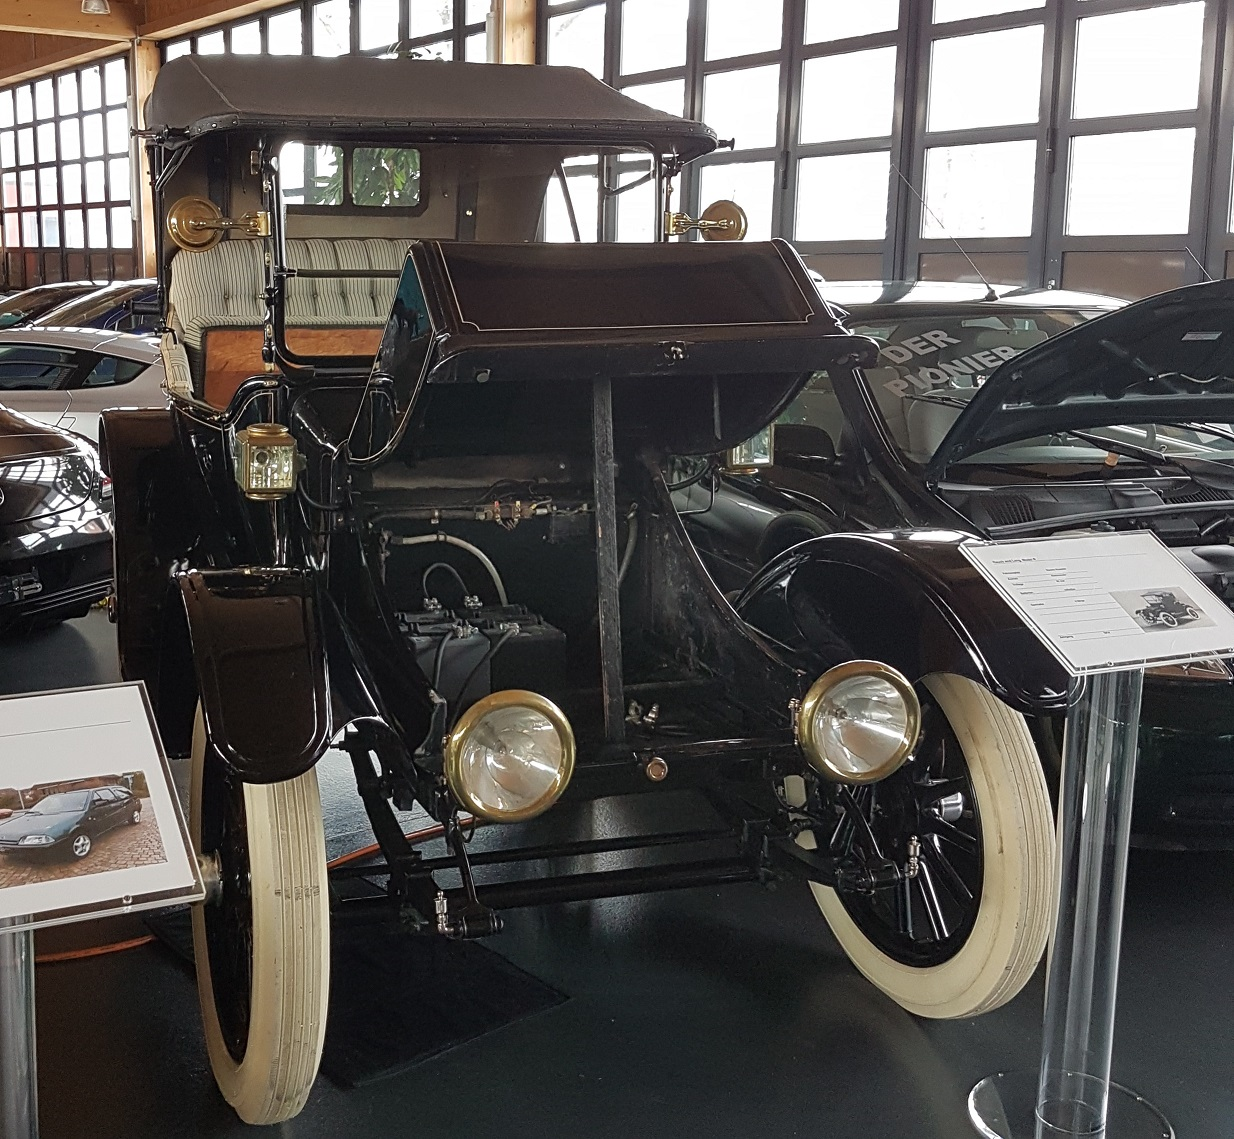
\includegraphics[width=0.8\textwidth]{images/Setz.JPG}
	\caption{Der Rauch und Lang im Museum von Herr Setz}
	\label{fig:Setz}
\end{figure}

Dadurch, dass in beinahe allen Stufen ein zusätzlicher Widerstand zum Motor geschaltet ist, entstehen zusätzliche Verluste im Auto, was die maximale Reichweite reduziert. Auch ist diese Schaltung nicht viel einfacher aufgebaut als die Schaltung des Detroits, lediglich die Auftrennung auf zwei Batterien entfällt. Anstelle der zusätzlichen Motoranzapfungen für die Feldansteuerungen sind in dieser Schaltung weitere Widerstände nötig. Das Verständnis der Schaltung ist aber bedeutend einfacher: Ein grösserer Widerstand in Serie behindert den Stromfluss zum Motor stärker als ein kleiner Widerstand, sodass durch sehr einfach die Leistung reguliert werden kann. Im Gegensatz zur Schaltung des Detroits steigen aber hier das maximale Moment und die erreichbare Geschwindigkeit (bei gegebenem Gegenmoment) mit den höheren Stufen an, da der serielle Widerstand sowohl den maximalen Strom limitiert (beziehungsweise den Stromfluss entsprechend verhindert), als auch die maximal induzierte Spannung bei gegebenem Strom verringert.